%%%%%%%%%%%%%%%%%%%%%%%%%%%%%%%%%%%%%%%%%%%%%%%%%%%%%%%%%%%%%
%
% Section: Foundations of Functions Review Questions
%
%%%%%%%%%%%%%%%%%%%%%%%%%%%%%%%%%%%%%%%%%%%%%%%%%%%%%%%%%%%%%

\section{Foundations of Functions Review Questions}

\subsection*{Function Terminology}
Each of the following relationships can be represented by a function. For each relationship
\begin{enumerate}[label=(\alph*)]
	\item state the input variable and quantity, 
	\item state the output variable and quantity, 
	\item describe the relationship as a function using the phrasing \quotes{\underline{\phantom{blank}} is a function of \underline{\phantom{blank}}} using both the variables and the quantities they represent, and 
	\item write an equation which relates the variables and the function.
\end{enumerate}
You may find it helpful to draw a function diagram.
\bigskip

\ex{The price $P$ for a gallon of gas can be determined by the number of days since a significant world event, $D$. The function used to determine this is called $G$.}
\sol{
	\begin{enumerate}[label=(\alph*)]
		\item Input: Number of days since significant world event, $D$
		\item Output: Price of a gallon of gas, $P$
		\item Relationship: The price of a gallon of gas is a function of the number of days since a significant world event; $P$ is a function of $D$
		\item Equation: $P = G(D)$
	\end{enumerate}
}

\bigskip
\ex{The number of hours of sleep, $h$, a new parent gets per night is determined by the age of a newborn, $w$, measured in weeks. The function used to determine this is called $s$.}
\sol{
	\begin{enumerate}[label=(\alph*)]
		\item Input: Age of newborn in weeks, $w$
		\item Output: Hours of sleep per night, $h$
		\item Relationship: The number of hours of sleep a new parent gets is a function of the age of a newborn; $h$ is a function of $w$
		\item Equation: $h = s(w)$
	\end{enumerate}
}

\bigskip
\ex{The function $c$ outputs the number of new positive covid cases per day, $p$, as a result of days since a new variant first emerges, $d$.}
\sol{
	\begin{enumerate}[label=(\alph*)]
		\item Input: Days since new variant emerges, $d$
		\item Output: Number of new positive covid cases per day, $p$
		\item Relationship: The number of new positive covid cases per day is a function of the number of days since a new varient emerges; $p$ is a function of $d$
		\item Equation: $p = c(d)$
	\end{enumerate}
}

\bigskip
\ex{The total profit, $p$, a company earns is determined by how many products it sells, $s$, using the function $c$.}
\sol{
	\begin{enumerate}[label=(\alph*)]
		\item Input: Number of products sold, $s$
		\item Output: Total profit earned, $p$
		\item Relationship: The total profit earned by a company is a function of how many products it sells; $p$ is a function of $s$
		\item Equation: $p = c(s)$
	\end{enumerate}
}

\bigskip
\ex{The amount of yarn, $y$, needed to knit a scarf is based on the size, $s$, using the function $k$. }
\sol{
	\begin{enumerate}[label=(\alph*)]
		\item Input: Size of scarf, $s$
		\item Output: Amount of yarn needed, $y$
		\item Relationship: The amount of yarn you need for a scarf is a function of the size of the scarf; $y$ is a function of $s$
		\item Equation: $y = k(s)$
	\end{enumerate}
}

\bigskip
\ex{The amount time, $t$, needed to get to your destination depends on the distance you are driving, $d$, using the function $m$. }
\sol{
	\begin{enumerate}[label=(\alph*)]
		\item Input: Distance you are driving, $d$
		\item Output: Time needed to get to destination, $t$
		\item Relationship: The time needed to get to your destination is a function of the distance you are driving; $t$ is a function of $d$
		\item Equation: $t = m(d)$
	\end{enumerate}
}

\bigskip
\noindent In each of the following problems, two variables and the quantities they represent are given, and an equation relating these variables with a function is also given.
\begin{enumerate}[label=(\alph*)]
	\item State the input variable and quantity, 
	\item State the output variable and quantity, and 
	\item describe the relationship using both the variables and the quantities they represent using the phrasing \quotes{\underline{     } a function of \underline{     }}.
\end{enumerate} 

\bigskip
\ex{$m$ is the number of minutes needed to commute to campus, $d$ is the distance to campus in miles, and $m=f(d)$.}
\sol{
	\begin{enumerate}[label=(\alph*)]
		\item Input: Distance to campus in miles, $ d $
		\item Output: Number of minutes needed to commute to campus, $ m $
		\item Relationship: The number of minutes needed to commute to campus is a function of the distance in miles to campus; $ m $ is a function of $ d $
	\end{enumerate}
} 

\bigskip
\ex{$ y $ is the number of years needed to save $ d $ dollars. $ s(d) = y $.}
\sol{
	\begin{enumerate}[label=(\alph*)]
		\item Input: Amount of money needed in dollars, $ d $
		\item Output: Number of years needed to save, $ y $
		\item Relationship: The number of years needed to save is a function of the amount of money needed; $ y $ is a function of $ d $
	\end{enumerate}
}

\bigskip
\ex{The interest rate for an auto loan, $ I $, an individual qualifies for is dependent on their credit score, $ C $. $ A(C) = I $.}
\sol{
	\begin{enumerate}[label=(\alph*)]
		\item Input: Credit score, $ C $
		\item Output: Interest rate for auto loan, $ I $
		\item Relationship: The interest rate for any auto loan is a function of their credit score; $ I $ is a function of $ C $
	\end{enumerate}
}

\bigskip
\ex{$ C $ is the wind chill resulting from the speed of the wind, $ w $. $ f(w) = C $.}
\sol{
	\begin{enumerate}[label=(\alph*)]
		\item Input: Wind speed, $ w $
		\item Output: Wind chill, $ C $
		\item Relationship: The wind chill is a function of the wind speed; $ C $ is a function of $ w $
	\end{enumerate}
}

\subsection*{Functions and Formulas}
\bigskip
\ex{ If $f(x) = 5x - 10$, find $f(3)$.}
\sol{$f(3)=5$}

\bigskip
\ex{ If $b(p) = p^2 - p + 1$, find $b(-4)$.}
\sol{$b(-4) = 21$}

\bigskip
\ex{ If $g(h) = h + 2$, find $g(-1)$.}
\sol{$g(-1) = -1$}

\bigskip
\ex{ If $d(t) = -2t^2 + t - 4$, find $d(-2)$.}
\sol{$d(-2) = -14$}

\bigskip
\ex{ If $a(b) = 7 - 4b$, find $a(-6)$.}
\sol{$a(-6) = 31$}

\bigskip
\ex{ If $c(d) = d^2 - 4d$, find $c(-1)$.}
\sol{$c(-1) = 5$}

\bigskip
\ex{ If $f(g) = \frac{g+6}{2g-4}$, find $f(0)$.}
\sol{$f(0) = -1.5$}

\bigskip
\ex{ The height (in meters) of a diver jumping off a 10-meter platform $t$ seconds after jumping is given by $h(t) = -4.9t^2 + 4t + 10$. Evaluate $h(1.2)$ and write a sentence interpreting the result.}
\sol{At $1.2$ seconds, the diver is at $7.744$ meters.}

\bigskip
\ex{ The amount of federal income tax an individual making less than $\$9,950$ pays can be calculated by the function $t(I) = 0.10I$. Use the function to determine the federal income tax for someone who made $\$5,000$.}
\sol{$t(5000) = 500$}

\subsection*{Determining Whether or Not a Rule is a Function}

\bigskip
Each of the following exercises describes a rule which could be used to process information. Determine whether or not the given rule is a function. Clearly justify your answer.
\bigskip
\ex{Let $u$ be the rule that assigns the UPC code to each item for sale in Wegmans.}
\sol{Yes}

\bigskip
\ex{Let $f$ be the rule that assigns the item being sold to the store 5 Below.}
\sol{No}

\bigskip
\ex{Let $g$ be the rule that gives the current GPA of each student at FLCC.}
\sol{Yes}

\bigskip
\ex{$M$ is the rule that gives the menu item for a specific restaurant.}
\sol{No}

\bigskip
\ex{$C$ is the rule that gives the eye color for each person getting an eye exam.}
\sol{Yes}

\bigskip
\ex{$P$ is the rule that assigns a textbook its length, in pages.}
\sol{Yes}

\bigskip
\ex{$g(a) = a^2 - 3$}
\sol{Yes}

\bigskip
\ex{$y = 5 - 3x$}
\sol{Yes}

\subsection*{Domain and Range}

\bigskip
\ex{ Let $g$ be the rule that gives the birthday of each living person born in the United States. What is the domain of $g$? What is the range of $g$?}
\sol{Domain: All US residents. Range: Jan 1 - Dec 31.}

\bigskip
\ex{ Let $r$ be the rule that gives the shoe size of each person renting bowling shoes on a given day. What is the domain of $r$? What is the range of $r$?}
\sol{Domain: Bowlers. Range: Possible shoe sizes.}

\bigskip
\ex{ $S$ is the rule that assigns a Social Security number to each citizen of the United States. What is the domain of $S$? What is the range of $S$?}
\sol{Domain: All US citizens. Range: All possible 9-digit combinations.}

\bigskip
\ex{ What is the domain of $f(x) = 3x - 4$?}
\sol{Domain: All real numbers}

\bigskip
\ex{ What is the domain of $g(t) = -2t^2 - t + 1$?}
\sol{Domain: All real numbers}

\bigskip
\ex{ What is the domain of $f(d) = \frac{2d+1}{d}$?}
\sol{Domain: All real numbers except $0$, $d \neq 0$}

\bigskip
\ex{ What is the domain of $r(q) = \sqrt{q-1}$?}
\sol{$q \geq 1$}

\bigskip
\ex{ What is the domain of $w(s) = \frac{s+2}{s-2}$?}
\sol{Domain: All real numbers except $2$, $s \neq 2$}

\bigskip
\ex{ What is the domain of $f(x) = \sqrt{2x - 4}$?}
\sol{$x \geq 2$}

\subsection*{Functions and Graphs}

\bigskip
\ex{Rewrite the function given below as a set of coordinate pairs.
	\begin{center}	
		$\begin{array}{c|cccc}
			x & 4 & 5 & 6 & 7 \\
			\hline
			f(x) & -1 & -2 & 0 & 4 \\
		\end{array}$
	\end{center}
}	
\sol{$(4,-1)$, $(5,-2)$, $(6,0)$, $(7,4)$}

\bigskip
\ex{For the following function notation, rewrite as a coordinate pair:
	\begin{enumerate}[label=(\alph*)]
		\item $g(3) = 5$
		\item $g(4) = -2$
		\item $a(-3) = 4$
		\item $10 = b(2)$
	\end{enumerate}
}
\sol{a.  $(3,5)$\\b.  $(4,-2)$\\c.  $(-3,4)$\\d.  $(2,10)$}

\bigskip
\ex{For the following coordinate pairs, rewrite using function notation, assume $f(x)$:
	\begin{enumerate}[label=(\alph*)]
		\item $(3,7)$
		\item $(-1,0)$
		\item $(8, -1)$
		\item $(3.5,7)$
		\item $(-100, 3)$
	\end{enumerate}
}
\sol{a.  $f(3)=7$\\b.  $f(	-1)=0$\\c.  $f(8)=-1$\\d.  $f(3.5)=7$\\e.  $f(-100)=\frac{3}{4}$}

\bigskip
\ex{Use your calculator to create a table of values for the function $f(x) = x^2 - 2x + 1$ for $x = -8, -6, -4, -2, 0, 2, 4, 6$. Sketch a coordinate plane and plot the points on your graph.
}
\sol{
	\begin{tabular}{c|c}
		$x$ & $f(x)$\\
		\hline
		$-8$ & $81$\\
		$-6$ & $49$\\
		$-4$ & $25$\\
		$-2$ & $9$\\
		$0$ & $1$\\
		$2$ & $1$\\
		$4$ & $9$\\
		$6$ & $25$
	\end{tabular}
	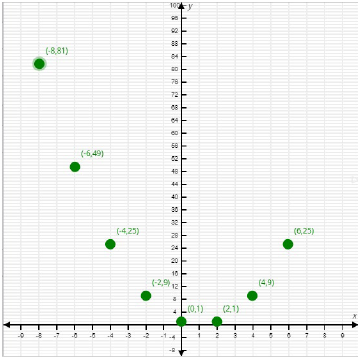
\includegraphics[scale=1.0]{Sections/FunctionsReviewQuestionsImages/Question39Figure01.png}
}

\bigskip
\ex{Use your calculator to create a table of values of the function $g(x) = x^2 - 3x - 4$ for $x = -4, -2, 0, 2, 4$, or create the table yourself by hand. Then sketch a coordinate plane and plot these points on it. Use the points you plotted to sketch what the graph of $g(x)$ appears to be.
}
\sol{
	\begin{tabular}{c|c}
		$x$ & $f(x)$\\
		\hline
		$-4$ & $24$\\
		$-2$ & $6$\\
		$0$ & $-4$\\
		$2$ & $-6$\\
		$4$ & $0$\\
	\end{tabular}
	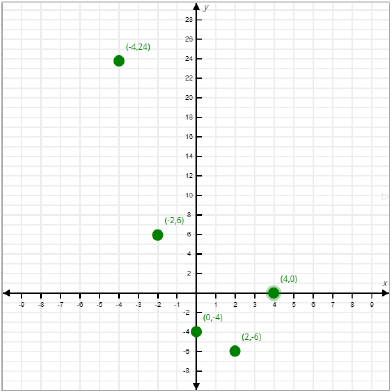
\includegraphics[scale=1.0]{Sections/FunctionsReviewQuestionsImages/Question40Figure01.png}
}

\bigskip
\ex{In which quadrant do each of the following coordinate pairs lie:
	\begin{enumerate}[label=(\alph*)]
		\item $(-1,4)$
		\item $(2,-7)$
		\item $(-9,-10)$
		\item $(5,0)$
	\end{enumerate}
}
\sol{a.  II\\b.  IV\\c.  III\\d.  None (between I and IV)}

\bigskip
\ex{Is $\{(4,2), (-10,4), (6, -3), (2,4), (-2, -1)\}$ a function? Why or why not?}
\sol{Yes}

\bigskip
\ex{Is $\{(-3,4), (6,9), (5,-7), (4,-3), (6,6)\}$ a function? Why or why not?}
\sol{No}

\bigskip
\ex{Use your calculator to obtain a graph for the function $p(x) = 5 - \frac{x}{4}$ in the standard window. Use your graph to find $p(2)$, $p(-2.5)$, and $p(3.9)$.}
\sol{$p(2)=4.5$, $p(-2.5)=5.625$, $p(3.9)=4.025$}

\bigskip
\ex{Use your calculator to obtain a graph for the function $r(n) = -4n^2 - 10n - 3$ in the window $-3 \leq n \leq 3$, $-100 \leq r(n) \leq -20$. Use your graph to find $r(1.33)$ and $r(-2.9)$.}
\sol{$r(1.33)=-23.3756$, $r(-2.9)=-7.64$}

\bigskip
\ex{Sketch a possible graph for the following scenarios, labeling axes and any other important information:
	\begin{enumerate}[label=(\alph*)]
		\item The amount of snowfall as a function of time during a blizzard.
		\item The sales of sunscreen as a function of time since the start of the year in New York State.
		\item The amount of food a caterer plans to make as a function of how many people are attending a wedding.
	\end{enumerate}
}
\sol{Answers will vary.\\a.  The graph should be generally increasing at potentially variable rates leveling off at the end of the blizzard.\\b.  The graph should increase through the spring and summer and decrease into the fall and winter.\\c.  The graph should increase at a constant rate.}

\bigskip
\ex{Are the following graphs of possible functions?\\
	\begin{tabular}{lll}
		a. 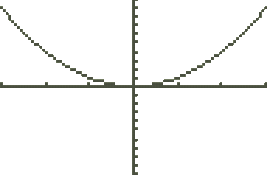
\includegraphics[scale=0.6]{Sections/FunctionsReviewQuestionsImages/Question48Figure01.png}
		&  	
		b. 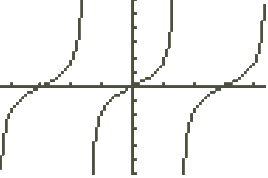
\includegraphics[scale=0.6]{Sections/FunctionsReviewQuestionsImages/Question48Figure02.png}
		&
		c. 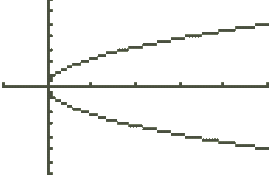
\includegraphics[scale=0.6]{Sections/FunctionsReviewQuestionsImages/Question48Figure03.png}
	\end{tabular}
}
\sol{a.  Yes\\b.  Yes\\c.  No}

\subsection*{Solve Graphically}

Solve each of the following equations graphically. You may need to adjust your window settings. Equations many have more than one solution. Round your answers
to two decimal places if necessary.

\bigskip
\ex{$5a - 15 = 70 - 2a$}
\sol{$a=\frac{85}{7} \approx 12.14$}

\bigskip
\ex{$50 = b^2 - b + 4$}
\sol{$b=-6.3$ or $b=7.3$}

\bigskip
\ex{$\frac{c^2}{4} = \frac{2c - 7}{2}$}
\sol{No solution}

\bigskip
\ex{$2.3(1.2d - 8) + 5.6d = 0.5 - 2.49(d + 7.1)$}
\sol{$d=0.11$}

\bigskip
\ex{$2x + 7 = 3x - 2$}
\sol{$x=9$}

\bigskip
\ex{$6t - 10 = -3t + 12$}
\sol{$t=\frac{22}{9} \approx 2.4$}

\bigskip
\ex{$0.36h - 7(1.2h + 4) = 0.98(1.8h - 1)$}
\sol{$h=\frac{6755}{2451} \approx -2.76$}

\bigskip
\ex{$\frac{4x+2}{5} = \frac{2x-1}{7}$}
\sol{$x=-\frac{19}{18} \approx -1.06$}

\bigskip
\ex{$\frac{6x+9}{2} = \frac{4x+1}{3} + 12$}
\sol{$x=\frac{47}{10}=4.7$}

\subsection*{Function Models}

\bigskip
For the following, evaluate and state your answers in ordinary English.

\bigskip
\ex{The cost to print a textbook is a function of the length (number of pages) and can be calculated using the function $c(p) = 6.50 + 0.10p$. What will be the total cost if the textbook is $400$ pages long?}
\sol{$c(400)=46.50$; The total cost to print a $400$ page textbook is $\$46.50$.}

\bigskip
\ex{You are on salary and get paid a set amount per week for working $40$ hours, and on top of that get paid a certain dollar amount for each hour you work over $40$ hours. Your weekly take home pay can be calculated using the function $p(h) = 600 + 25(h-40)$. How many hours did you work if your weekly take home pay was $\$975.00$?}
\sol{$h=55 hours$; If you got paid $\$975$ dollars, then you worked $55$ hours that week.}

\bigskip
\ex{A batter hits a baseball and the ball’s height, in feet, after $t$ seconds is given by the function $h(t) = -16t^2 + 140t + 3$. What is the ball’s height $6$ seconds after the batter hits it?}
\sol{$h(6)=267$; The height of the ball was $267$ feet $6$ seconds after being hit.}

\bigskip
\noindent Give an interpretation in ordinary English for the following information given in function notation:
\bigskip
\ex{The cost to host my child’s birthday party at a bowling alley is a function of the number of children she invites. Interpret $f(9) = 150$.}
\sol{If $9$ children are invited, then the cost is $\$150.00$}

\bigskip
\ex{A student’s score on a unit exam is a function of the number of points they earned out of fifty. Interpret $f(45) = 90$.}
\sol{On the unit exam, $45$ points earned out of $50$, yields a $90\%$.}

\bigskip
\ex{The temperature in degrees Fahrenheit is a function of the temperature in degrees Celsius. Interpret $f(0) = 32$.}
\sol{$0^\circ$C=$32^\circ$F}

\bigskip
\noindent Express the following information using function notation.
\bigskip
\ex{The amount due for this monthly cell phone plan is a function $f$ of the number of minutes the customer used. $\$45.90$ was due when $120$ minutes were used.}
\sol{$f(120)=45.9$}

\bigskip
\ex{The distance a runner has traveled is a function $r$ of the time, in minutes, she has been running. A runner has traveled $6$ miles after running $60$ minutes.}
\sol{$r(60)=6$}

\bigskip
\ex{The cost to purchase a large pizza is a function $c$ of how many toppings you add. I added $4$ toppings and my pizza cost $\$27.00$.}
\sol{$c(4)=27$}

\bigskip
\noindent For the following scenarios give the relevant domain and relevant range:
\bigskip
\ex{The amount of rain in my rain barrel, in inches, is a function of the number of hours in a day it has been raining.}
\sol{Domain: $0 \leq h \leq 24$, Range: $0 \leq r \leq 12$}

\bigskip
\ex{The amount of people that are allowed to attend a church service is a function of the number of seats available.}
\sol{Domain: $0 \leq s \leq 300$, Range: $0 \leq p \leq 300$}

\bigskip
\ex{A girl scout is selling cookies for $\$5$ a box. Her profits for selling $c$ number of boxes can be calculated using the function $g(c) = 5c - 20$. Give a reasonable relevant domain and relevant range for this function.}
\sol{Domain: $0 \leq c \leq 50$, Range: $0 \leq g(c) \leq 230$}

\subsection*{Implicit Functions}

\bigskip
\ex{Solve the equation $3x - 5y = 7$ explicitly for $y$.}
\sol{$y=\frac{7-3x}{-5}=\frac{3x-7}{5}$}

\bigskip
\ex{Solve the equation $3x - 5y = 7$ explicitly for $x$.}
\sol{$x=\frac{5y+7}{3}$}

\bigskip
\ex{Rewrite the equation so $y$ is a function of $x$: $2(4x - 7) - 8y = -3(y - 1)$.}
\sol{$y=\frac{8x-17}{5}$}

\bigskip
\ex{Rewrite the equation so $m$ is a function of $n$: $\frac{m}{2} - 6 = n$.}
\sol{$m=2(n+6)=2n+12$}

\bigskip
\ex{Rewrite the equation so $p$ is a function of $q$: $\frac{p - 6}{2} = q + 8$.}
\sol{$p=2(q+8)=2q+16$}

\bigskip
\ex{Solve the equation for $j$: $p = \frac{j + 9}{15}$.}
\sol{$j=15p-9$}

\subsection*{Rates of Change}

\bigskip
\ex{
	The table below gives average price of a gallon of gas in NYS in January of each year.
	$$
	\begin{array}{c|c}
		\hline
		\text{Year} & \text{Price per gallon} \\
		\hline
		2015 & 2.51 \\
		2019 & 2.44 \\
		2021 & 2.35 \\
		2022 & 3.42 \\
		\hline
	\end{array}
	$$
	\begin{enumerate}[label=(\alph*)]
		\item What is the average rate of change (AROC) from 2015 to 2022?
		\item What is the average rate of change (AROC) from 2015 to 2021?
		\item What is the average rate of change (AROC) from 2019 to 2021?
		\item Write a sentence interpreting the AROC from part (b).
	\end{enumerate}
}
\sol{a.  $\$0.13 / year$\\b.  $\$-.07/year$\\c.  $-0.05/year$\\d.  Between 2015 and 2022 the price of a gallon of gasoline dropped an average of $\$0.03$ per year.}

\bigskip
\ex{
	The table below gives the number of kilotons of $\text{CO}_2$ emitted by the United States.
	$$
	\begin{array}{c|c}
		\hline
		\text{Year} & \text{kilotons of CO}_2 \\
		\hline
		2015 & 4,982,790 \\
		2017 & 4,813,720 \\
		\hline
	\end{array}
	$$
	Calculate the AROC and write a sentence interpreting the result.}
\sol{$-84,535$; The amount of $\text{CO}_2$ has dropped an average of $84,535$ kilotons per year. }

\bigskip
\ex{Rachel is driving to visit her mother and her distance from home is a function of how many hours she has been driving. After $5$ hours she is $325$ miles from her house. After $10$ hours she is $635$ miles from her house. Find the average rate of change in her distance from home between $5$ hours and $10$ hours of her driving. Do you expect this rate to remain constant over the course of her entire trip?}
\sol{$62mph$}

\bigskip
\ex{
	When Ben was 5-years old he was $36$ inches tall. Ben is now 8-years old and is $44$ inches tall. Find the average rate of change in Ben’s height as a function of his age. Do you expect this rate to remain constant over time?}
\sol{$2.7$ ins/year; No.}

\bigskip
\ex{A pizza place offers a special on a large cheese pizza plus extra per topping added. I ordered a large pizza with $2$ toppings and the total (before tax) was $\$17$. My sister ordered a large pizza with $4$ toppings and her total (before tax) was $\$19$. Find the average rate of change in cost as a function of the number of toppings ordered on the pizza. Do you expect this rate to remain constant?}
\sol{$\$1.00$/topping; yes}

\bigskip
\ex{Find the AROC of the function $f(x) = 9 - x^2$ between $x = -2$ and $x = 3$.}
\sol{$-1$}

\bigskip
\ex{Find the AROC of the function $g(x) = 5 - (x + 2)$ between $x = 2$ and $x = 7$.}
\sol{$-1$}

\bigskip
\ex{Find the average rate of change in the function $g(t) = 2t - 4$ between $t = 0$ and $t = 5$.}
\sol{$2$}

\bigskip
\ex{Find the average rate of change in the function $f(x) = x^2 - 2x + 1$ between $x = 3$ and $x = 7$.}
\sol{$8$}

\bigskip
\ex{Find the average rate of change in the function $h(w) = \frac{3w - 4}{w}$ between $w = -1$ and $w = 2$.}
\sol{$-2$}

\clearpage
